\documentclass[]{article}
\usepackage{lmodern}
\usepackage{amssymb,amsmath}
\usepackage{ifxetex,ifluatex}
\usepackage{fixltx2e} % provides \textsubscript
\ifnum 0\ifxetex 1\fi\ifluatex 1\fi=0 % if pdftex
  \usepackage[T1]{fontenc}
  \usepackage[utf8]{inputenc}
\else % if luatex or xelatex
  \ifxetex
    \usepackage{mathspec}
  \else
    \usepackage{fontspec}
  \fi
  \defaultfontfeatures{Ligatures=TeX,Scale=MatchLowercase}
\fi
% use upquote if available, for straight quotes in verbatim environments
\IfFileExists{upquote.sty}{\usepackage{upquote}}{}
% use microtype if available
\IfFileExists{microtype.sty}{%
\usepackage{microtype}
\UseMicrotypeSet[protrusion]{basicmath} % disable protrusion for tt fonts
}{}
\usepackage[margin=1in]{geometry}
\usepackage{hyperref}
\hypersetup{unicode=true,
            pdftitle={Non-disclosive federated omic data analysis with DataSHIELD and Bioconductor},
            pdfborder={0 0 0},
            breaklinks=true}
\urlstyle{same}  % don't use monospace font for urls
\usepackage{color}
\usepackage{fancyvrb}
\newcommand{\VerbBar}{|}
\newcommand{\VERB}{\Verb[commandchars=\\\{\}]}
\DefineVerbatimEnvironment{Highlighting}{Verbatim}{commandchars=\\\{\}}
% Add ',fontsize=\small' for more characters per line
\usepackage{framed}
\definecolor{shadecolor}{RGB}{248,248,248}
\newenvironment{Shaded}{\begin{snugshade}}{\end{snugshade}}
\newcommand{\AlertTok}[1]{\textcolor[rgb]{0.94,0.16,0.16}{#1}}
\newcommand{\AnnotationTok}[1]{\textcolor[rgb]{0.56,0.35,0.01}{\textbf{\textit{#1}}}}
\newcommand{\AttributeTok}[1]{\textcolor[rgb]{0.77,0.63,0.00}{#1}}
\newcommand{\BaseNTok}[1]{\textcolor[rgb]{0.00,0.00,0.81}{#1}}
\newcommand{\BuiltInTok}[1]{#1}
\newcommand{\CharTok}[1]{\textcolor[rgb]{0.31,0.60,0.02}{#1}}
\newcommand{\CommentTok}[1]{\textcolor[rgb]{0.56,0.35,0.01}{\textit{#1}}}
\newcommand{\CommentVarTok}[1]{\textcolor[rgb]{0.56,0.35,0.01}{\textbf{\textit{#1}}}}
\newcommand{\ConstantTok}[1]{\textcolor[rgb]{0.00,0.00,0.00}{#1}}
\newcommand{\ControlFlowTok}[1]{\textcolor[rgb]{0.13,0.29,0.53}{\textbf{#1}}}
\newcommand{\DataTypeTok}[1]{\textcolor[rgb]{0.13,0.29,0.53}{#1}}
\newcommand{\DecValTok}[1]{\textcolor[rgb]{0.00,0.00,0.81}{#1}}
\newcommand{\DocumentationTok}[1]{\textcolor[rgb]{0.56,0.35,0.01}{\textbf{\textit{#1}}}}
\newcommand{\ErrorTok}[1]{\textcolor[rgb]{0.64,0.00,0.00}{\textbf{#1}}}
\newcommand{\ExtensionTok}[1]{#1}
\newcommand{\FloatTok}[1]{\textcolor[rgb]{0.00,0.00,0.81}{#1}}
\newcommand{\FunctionTok}[1]{\textcolor[rgb]{0.00,0.00,0.00}{#1}}
\newcommand{\ImportTok}[1]{#1}
\newcommand{\InformationTok}[1]{\textcolor[rgb]{0.56,0.35,0.01}{\textbf{\textit{#1}}}}
\newcommand{\KeywordTok}[1]{\textcolor[rgb]{0.13,0.29,0.53}{\textbf{#1}}}
\newcommand{\NormalTok}[1]{#1}
\newcommand{\OperatorTok}[1]{\textcolor[rgb]{0.81,0.36,0.00}{\textbf{#1}}}
\newcommand{\OtherTok}[1]{\textcolor[rgb]{0.56,0.35,0.01}{#1}}
\newcommand{\PreprocessorTok}[1]{\textcolor[rgb]{0.56,0.35,0.01}{\textit{#1}}}
\newcommand{\RegionMarkerTok}[1]{#1}
\newcommand{\SpecialCharTok}[1]{\textcolor[rgb]{0.00,0.00,0.00}{#1}}
\newcommand{\SpecialStringTok}[1]{\textcolor[rgb]{0.31,0.60,0.02}{#1}}
\newcommand{\StringTok}[1]{\textcolor[rgb]{0.31,0.60,0.02}{#1}}
\newcommand{\VariableTok}[1]{\textcolor[rgb]{0.00,0.00,0.00}{#1}}
\newcommand{\VerbatimStringTok}[1]{\textcolor[rgb]{0.31,0.60,0.02}{#1}}
\newcommand{\WarningTok}[1]{\textcolor[rgb]{0.56,0.35,0.01}{\textbf{\textit{#1}}}}
\usepackage{graphicx,grffile}
\makeatletter
\def\maxwidth{\ifdim\Gin@nat@width>\linewidth\linewidth\else\Gin@nat@width\fi}
\def\maxheight{\ifdim\Gin@nat@height>\textheight\textheight\else\Gin@nat@height\fi}
\makeatother
% Scale images if necessary, so that they will not overflow the page
% margins by default, and it is still possible to overwrite the defaults
% using explicit options in \includegraphics[width, height, ...]{}
\setkeys{Gin}{width=\maxwidth,height=\maxheight,keepaspectratio}
\IfFileExists{parskip.sty}{%
\usepackage{parskip}
}{% else
\setlength{\parindent}{0pt}
\setlength{\parskip}{6pt plus 2pt minus 1pt}
}
\setlength{\emergencystretch}{3em}  % prevent overfull lines
\providecommand{\tightlist}{%
  \setlength{\itemsep}{0pt}\setlength{\parskip}{0pt}}
\setcounter{secnumdepth}{0}
% Redefines (sub)paragraphs to behave more like sections
\ifx\paragraph\undefined\else
\let\oldparagraph\paragraph
\renewcommand{\paragraph}[1]{\oldparagraph{#1}\mbox{}}
\fi
\ifx\subparagraph\undefined\else
\let\oldsubparagraph\subparagraph
\renewcommand{\subparagraph}[1]{\oldsubparagraph{#1}\mbox{}}
\fi

%%% Use protect on footnotes to avoid problems with footnotes in titles
\let\rmarkdownfootnote\footnote%
\def\footnote{\protect\rmarkdownfootnote}

%%% Change title format to be more compact
\usepackage{titling}

% Create subtitle command for use in maketitle
\providecommand{\subtitle}[1]{
  \posttitle{
    \begin{center}\large#1\end{center}
    }
}

\setlength{\droptitle}{-2em}

  \title{Non-disclosive federated omic data analysis with DataSHIELD and
Bioconductor}
    \pretitle{\vspace{\droptitle}\centering\huge}
  \posttitle{\par}
    \author{true \\ true}
    \preauthor{\centering\large\emph}
  \postauthor{\par}
      \predate{\centering\large\emph}
  \postdate{\par}
    \date{2020-02-19}


\begin{document}
\maketitle

\hypertarget{purpose}{%
\section{Purpose}\label{purpose}}

The purpose of
\emph{\href{https://github.com/isgloba-brge}{dsOmicsClient}} is to
provide a set of functions to perform omic association analyses when
data are stored on federated databases or, more generally, in different
repositories. In particular the package utilizes DataSHIELD
infrastructure which is a software solution that allows for the
simultaneous co-analysis of data from multiple studies stored on
different servers without the need to physically pool data or disclose
sensitive information (Wilson et al. 2017). DataSHIELD uses
\href{http://opaldoc.obiba.org/en/latest/}{Opal servers} to properly
perform such analyses.

At a high level DataSHIELD is set up as a client-server model which
houses the data for a particular study. A request is made from the
client to run specific functions on the remote servers where the
analysis is performed. Non-sensitive and pre-approved summary statistics
are returned from each study to the client where they can be combined
for an overall analysis. An overview of what a single-site DataSHIELD
architecture would look like is illustrated in Figure
\ref{fig:dsArchitec}.

\begin{figure}

{\centering 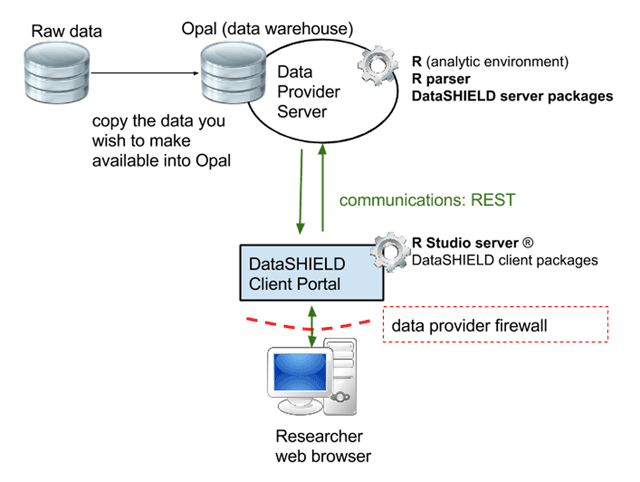
\includegraphics[width=0.9\linewidth]{fig/singleSiteDSInfrastructure} 

}

\caption{Single Server DataSHIELD Architecture (Wilson et al 2017)}\label{fig:dsArchitec}
\end{figure}

One of the main limitations of DataSHIELD is how to deal with large data
given the restrictions of Opal with databases. Nonetheless, the recent
development of the \emph{\href{https://github.com/obiba}{resourcer}} R
package allows DataSHIELD developers to overcome this drawback by
granting the Opal servers to deal with any type of data
(e.g.~\textbf{resources}). So far, Opal can register access to different
type of data resources in different formats (csv, tsv, R data, SQL,
tiddy, ..) that can also be located in different places (http, ssh, ASW
W3, local, \ldots). This is another important advancement since the
\emph{\href{https://github.com/obiba}{resourcer}} addresses another
important issue that is having duplicated data in diferent research
centers or hospitals.

The \emph{\href{https://github.com/obiba}{resourcer}} package permits to
work with specific R data classes. This is higly important in our
setting since it will allow to use
\href{www.bioconductor.org}{Bioconductor} classes to properly manage
omic data using efficient infrastructures such as \texttt{ExpressionSet}
or \texttt{RangedSummarizedExperiment} among others. Another important
asset of the \emph{\href{https://github.com/obiba}{resourcer}} package
is that it can be extended to new data types by writting specific
functions (see
\url{https://github.com/obiba/resourcer/\#extending-resources}). We have
use this feature and created some functions for the analysis of Variant
Calling Format (VCF files) that are loaded into R as Genomic Data
Storage objects. These functions along with others that allow the
managment of Bioconductor classes in DataSHIELD have been included in a
new DataSHIELD base package,
\emph{\href{https://github.com/isglobal-brge}{dsOmics}}, that is able to
manage different \href{www.bioconductor.org}{Bioconductor} data
infrastructures that are required to perform omic association analyses.
These including \texttt{ExpressionSet},
\texttt{RangedSummarizedExperiment} or \texttt{GDS} among others
\textbf{{[}what about HDF5, Yannick?{]}}.

In the next sections we first describe how to deal with Opal servers and
resources. We illustre how we prepared a test envioronment to describe
how Opal must be setup as well as how to provide the appropiate
R/DataSHILED configuration in both the Opal server and in the client
side to perform omic association analyses. Then, different the different
types of omic data analyses that can be perfomred with
\emph{\href{https://github.com/isgloba-brge}{dsOmicsClient}} are
described and further illustrated using real data examples including
epigenome, transcriptome and genomic data analyses.

\hypertarget{setup}{%
\section{Setup}\label{setup}}

\hypertarget{required-opal-server-with-resources}{%
\subsection{Required Opal server with
resources}\label{required-opal-server-with-resources}}

Resources are datasets or computation units which location is described
by a URL and access is protected by credentials. When assigned to a
R/DataSHIELD server session, remote big/complex datasets or high
performance computers are made accessible to data analysts.

Instead of storing the data in Opal's database, only the way to access
them is to be defined: the datasets are kept in their original format
and location (an R object, a SQL database, a SPSS file, etc.) and are
read directly from the R/DataSHIELD server-side session. Then as soon as
there is a R reader for the dataset or a connector for the analysis
services, a resource can be defined. Opal takes care of the DataSHIELD
permissions (a DS user cannot see the resource's credentials) and of the
resources assignment to a R/DataSHIELD session (see Figure
\ref{fig:resources})

\begin{figure}

{\centering 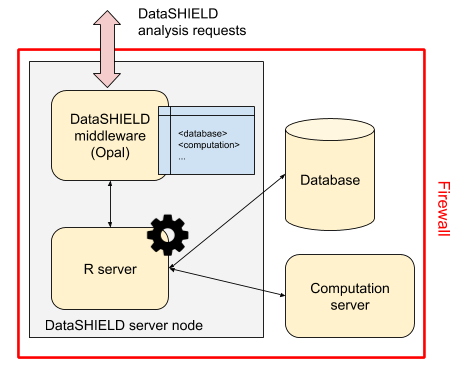
\includegraphics[width=0.9\linewidth]{fig/resourcer_fig} 

}

\caption{Resources: a new DataSHIELD infrastructure}\label{fig:resources}
\end{figure}

As previously mentioned, the \texttt{resourcer} R package allows to deal
with the main data sources (using tidyverse, DBI, dplyr, sparklyr,
MongoDB, AWS S3, SSH etc.) and is easily extensible to new ones
including specific data infrastructure in R or Bioconductor. So far
\texttt{ExpressionSet} and \texttt{RangedSummarizedExperiment} object
saved in \texttt{.rdata} files are accesible through the
\texttt{resourcer} package. The \texttt{dsOmics} package contains a new
extension that deals with VCF (Variant Calling Format) files which are
coerced to a GDS (Genomic Data Storage) format (VCF2GDS).

**{[}Yannick, do we have to write something here? or just indicate the
functions you created?{]}

We have prepared a test environment, with the Opal implementation of
Resources and an appropriate R/DataSHIELD configuration that is
available at: \url{https://opal-test.obiba.org}. This figure illustrate
the resources which are avaiable for the \texttt{test} project:

\begin{figure}

{\centering 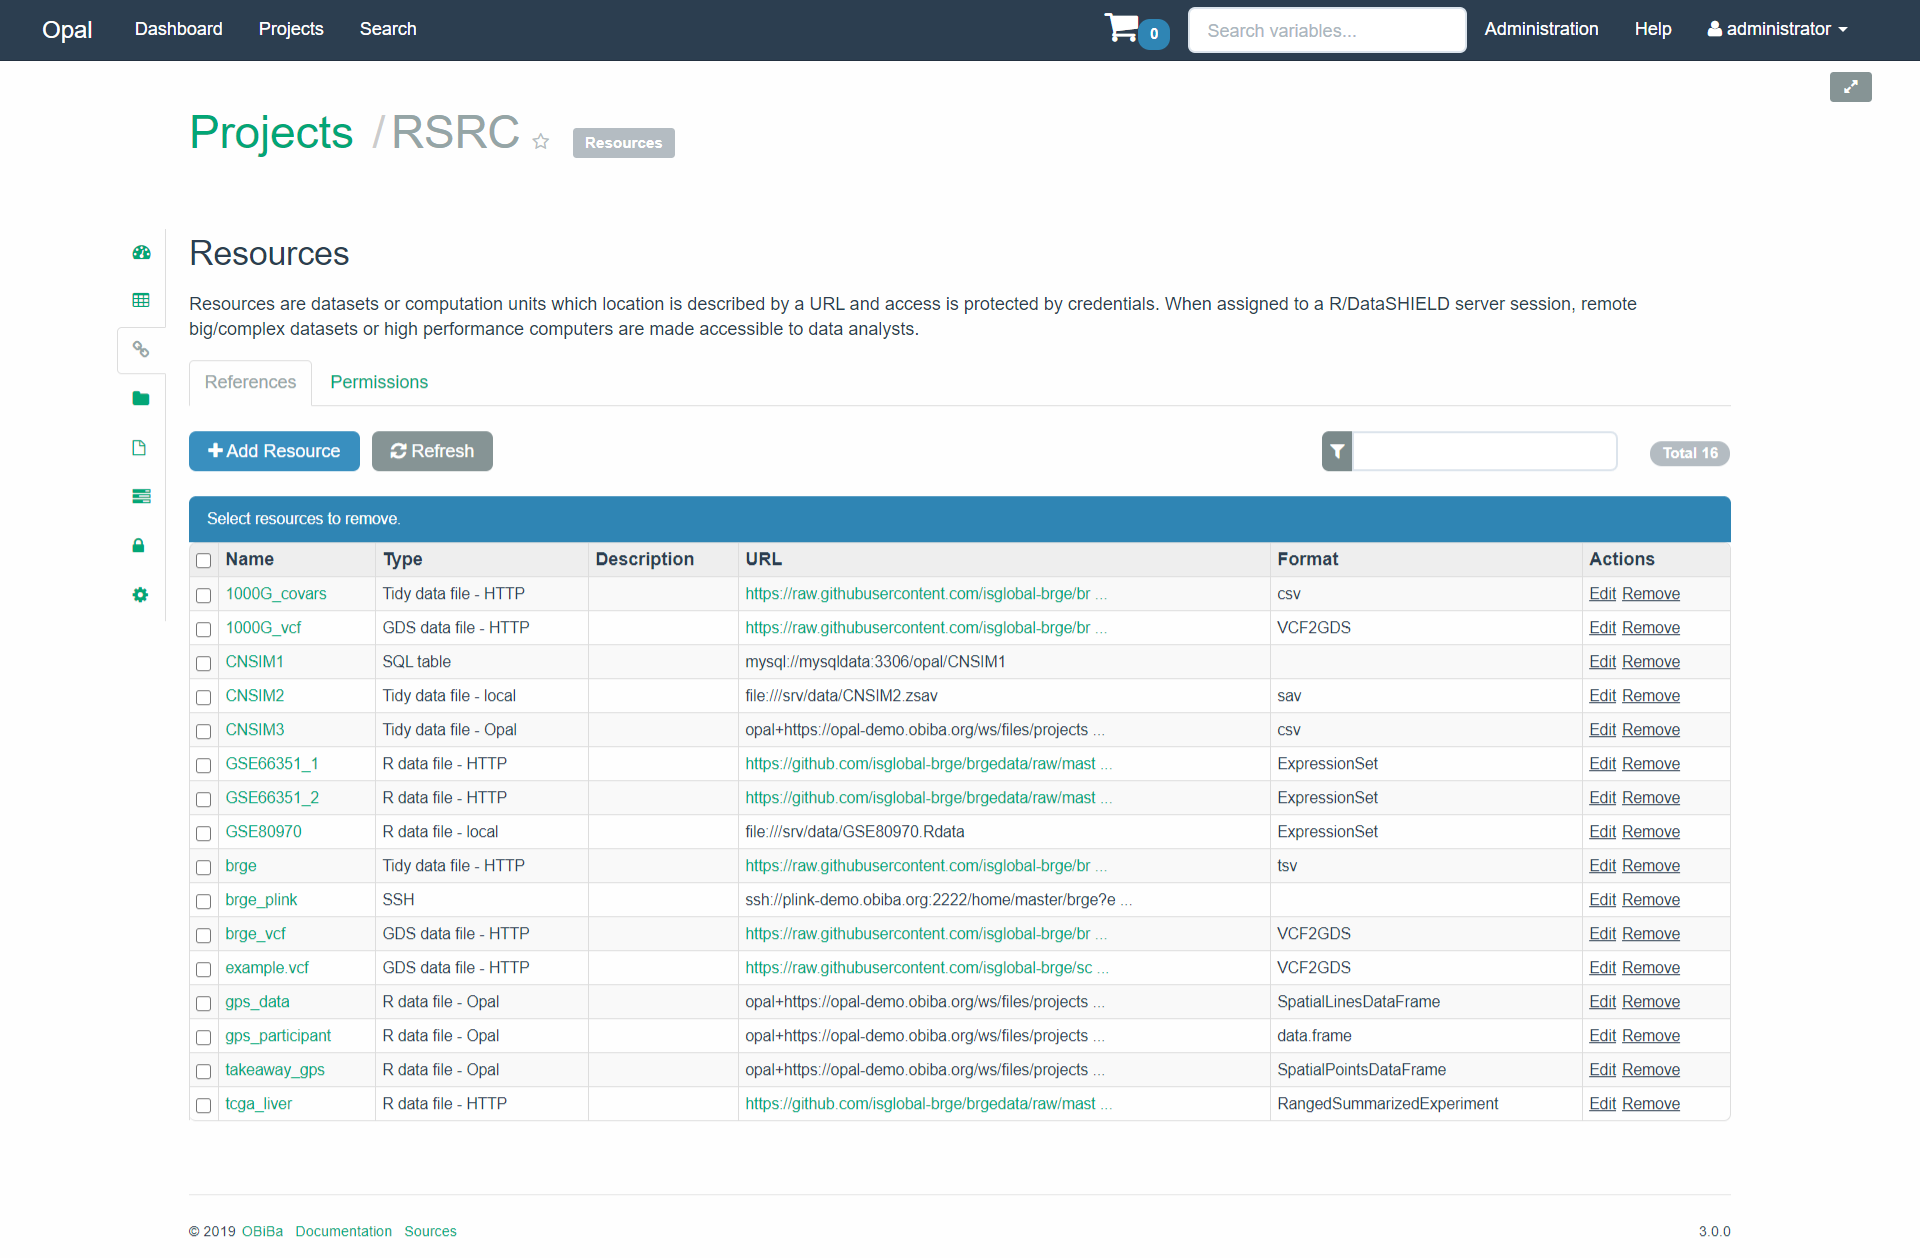
\includegraphics[width=25in]{fig/opal_resources} 

}

\caption{Resources from a test enviroment available at https://opal-test.obiba.org}\label{fig:testResources}
\end{figure}

It is possible to declare a resource that is to be resolved by an R
package that uses the \texttt{resourcer} API

\begin{figure}

{\centering 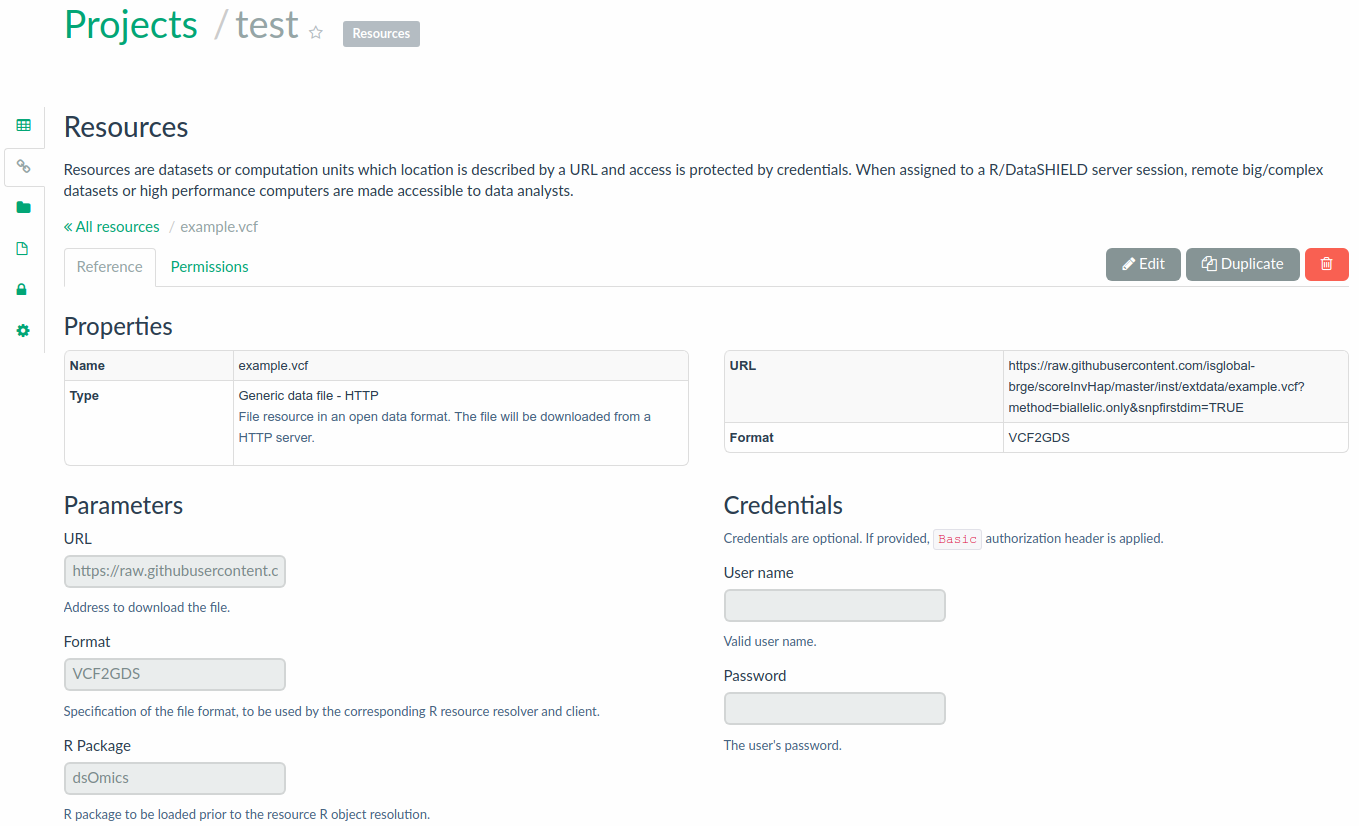
\includegraphics[width=28.14in]{fig/opal_resources_API} 

}

\caption{Declaration of a resource corresponding to a VCF2GDS format}\label{fig:testDeclaration}
\end{figure}

This can be automatically be done using R code by:

\begin{Shaded}
\begin{Highlighting}[]
\NormalTok{devtools}\OperatorTok{::}\KeywordTok{install\_github}\NormalTok{(}\StringTok{"obiba/opalr"}\NormalTok{, }\DataTypeTok{dependencies =} \OtherTok{TRUE}\NormalTok{)}
\end{Highlighting}
\end{Shaded}

\begin{Shaded}
\begin{Highlighting}[]
\OperatorTok{>}\StringTok{ }\KeywordTok{library}\NormalTok{(opalr)}
\OperatorTok{>}\StringTok{ }\NormalTok{o <{-}}\StringTok{ }\KeywordTok{opal.login}\NormalTok{(}\DataTypeTok{username =} \StringTok{"XXXXX"}\NormalTok{, }\DataTypeTok{password =} \StringTok{"XXXXX"}\NormalTok{, }
                  \DataTypeTok{url =} \StringTok{"https://opal{-}test.obiba.org"}\NormalTok{)}
\OperatorTok{>}\StringTok{ }\KeywordTok{opal.assign.resource}\NormalTok{(o, }\StringTok{"D"}\NormalTok{, }\DataTypeTok{value =} \StringTok{"test.example.vcf"}\NormalTok{)}
\OperatorTok{>}\StringTok{ }\KeywordTok{opal.execute}\NormalTok{(o, }\StringTok{"class(D)"}\NormalTok{)}
\NormalTok{[}\DecValTok{1}\NormalTok{] }\StringTok{"GDSFileResourceClient"} \StringTok{"FileResourceClient"}    \StringTok{"ResourceClient"}        \StringTok{"R6"}                   
\OperatorTok{>}\StringTok{ }\KeywordTok{opal.assign.script}\NormalTok{(o, }\StringTok{"G"}\NormalTok{, }\KeywordTok{quote}\NormalTok{(D}\OperatorTok{$}\KeywordTok{getValue}\NormalTok{()))}
\OperatorTok{>}\StringTok{ }\KeywordTok{opal.execute}\NormalTok{(o, }\StringTok{"class(G)"}\NormalTok{)}
\NormalTok{[}\DecValTok{1}\NormalTok{] }\StringTok{"gds.class"}
\OperatorTok{>}\StringTok{ }\KeywordTok{opal.execute}\NormalTok{(o, }\StringTok{"gdsfmt::diagnosis.gds(G)"}\NormalTok{)}
\OperatorTok{$}\NormalTok{stream}
\NormalTok{   id size capacity num\_chunk                    path}
\DecValTok{1}   \DecValTok{1}  \DecValTok{422}      \DecValTok{422}         \DecValTok{1}                \OperatorTok{/}\StringTok{ }\ErrorTok{$}\NormalTok{head}\OperatorTok{$}
\DecValTok{2}   \DecValTok{2}  \DecValTok{113}      \DecValTok{113}         \DecValTok{1}\NormalTok{        sample.id }\OperatorTok{$}\NormalTok{head}\OperatorTok{$}
\DecValTok{3}   \DecValTok{3}  \DecValTok{149}      \DecValTok{149}         \DecValTok{1}\NormalTok{        sample.id }\OperatorTok{$}\NormalTok{data}\OperatorTok{$}
\DecValTok{4}   \DecValTok{4}  \DecValTok{114}      \DecValTok{114}         \DecValTok{1}\NormalTok{           snp.id }\OperatorTok{$}\NormalTok{head}\OperatorTok{$}
\DecValTok{5}   \DecValTok{5}  \DecValTok{397}      \DecValTok{397}         \DecValTok{1}\NormalTok{           snp.id }\OperatorTok{$}\NormalTok{data}\OperatorTok{$}
\DecValTok{6}   \DecValTok{6}  \DecValTok{113}      \DecValTok{113}         \DecValTok{1}\NormalTok{        snp.rs.id }\OperatorTok{$}\NormalTok{head}\OperatorTok{$}
\DecValTok{7}   \DecValTok{7} \DecValTok{1757}     \DecValTok{1757}         \DecValTok{1}\NormalTok{        snp.rs.id }\OperatorTok{$}\NormalTok{data}\OperatorTok{$}
\DecValTok{8}   \DecValTok{8}  \DecValTok{114}      \DecValTok{114}         \DecValTok{1}\NormalTok{     snp.position }\OperatorTok{$}\NormalTok{head}\OperatorTok{$}
\DecValTok{9}   \DecValTok{9}  \DecValTok{793}      \DecValTok{793}         \DecValTok{1}\NormalTok{     snp.position }\OperatorTok{$}\NormalTok{data}\OperatorTok{$}
\DecValTok{10} \DecValTok{10}  \DecValTok{113}      \DecValTok{113}         \DecValTok{1}\NormalTok{   snp.chromosome }\OperatorTok{$}\NormalTok{head}\OperatorTok{$}
\DecValTok{11} \DecValTok{11}   \DecValTok{97}       \DecValTok{97}         \DecValTok{1}\NormalTok{   snp.chromosome }\OperatorTok{$}\NormalTok{data}\OperatorTok{$}
\DecValTok{12} \DecValTok{12}  \DecValTok{113}      \DecValTok{113}         \DecValTok{1}\NormalTok{       snp.allele }\OperatorTok{$}\NormalTok{head}\OperatorTok{$}
\DecValTok{13} \DecValTok{13}  \DecValTok{417}      \DecValTok{417}         \DecValTok{1}\NormalTok{       snp.allele }\OperatorTok{$}\NormalTok{data}\OperatorTok{$}
\DecValTok{14} \DecValTok{16}  \DecValTok{115}      \DecValTok{115}         \DecValTok{1}\NormalTok{        snp.annot }\OperatorTok{$}\NormalTok{head}\OperatorTok{$}
\DecValTok{15} \DecValTok{17}  \DecValTok{115}      \DecValTok{115}         \DecValTok{1}\NormalTok{   snp.annot}\OperatorTok{/}\NormalTok{qual }\OperatorTok{$}\NormalTok{head}\OperatorTok{$}
\DecValTok{16} \DecValTok{18}  \DecValTok{105}      \DecValTok{105}         \DecValTok{1}\NormalTok{   snp.annot}\OperatorTok{/}\NormalTok{qual }\OperatorTok{$}\NormalTok{data}\OperatorTok{$}
\DecValTok{17} \DecValTok{19}  \DecValTok{113}      \DecValTok{113}         \DecValTok{1}\NormalTok{ snp.annot}\OperatorTok{/}\NormalTok{filter }\OperatorTok{$}\NormalTok{head}\OperatorTok{$}
\DecValTok{18} \DecValTok{20}  \DecValTok{149}      \DecValTok{149}         \DecValTok{1}\NormalTok{ snp.annot}\OperatorTok{/}\NormalTok{filter }\OperatorTok{$}\NormalTok{data}\OperatorTok{$}
\DecValTok{19} \DecValTok{21}   \DecValTok{81}       \DecValTok{81}         \DecValTok{1}\NormalTok{         genotype }\OperatorTok{$}\NormalTok{head}\OperatorTok{$}
\DecValTok{20} \DecValTok{22} \DecValTok{2850}     \DecValTok{2850}         \DecValTok{1}\NormalTok{         genotype }\OperatorTok{$}\NormalTok{data}\OperatorTok{$}
\DecValTok{21} \OtherTok{NA}    \DecValTok{0}        \DecValTok{0}         \DecValTok{0}                \OperatorTok{$}\NormalTok{unused}\OperatorTok{$}

\ErrorTok{$}\NormalTok{log}
\NormalTok{ [}\DecValTok{1}\NormalTok{] }\StringTok{"Open a GDS file (File Version, major: 01, minor: 00)."}         \StringTok{"Load all data stream (20 in total) with an entry id (0x0001)."}
\NormalTok{ [}\DecValTok{3}\NormalTok{] }\StringTok{"Load the root folder from the entry (size: 422)."}              \StringTok{"==> / []"}                                                     
\NormalTok{ [}\DecValTok{5}\NormalTok{] }\StringTok{"==> / [dStr8]"}                                                 \StringTok{"==> / [dInt32]"}                                               
\NormalTok{ [}\DecValTok{7}\NormalTok{] }\StringTok{"==> / [dStr8]"}                                                 \StringTok{"==> / [dInt32]"}                                               
\NormalTok{ [}\DecValTok{9}\NormalTok{] }\StringTok{"==> / [dStr8]"}                                                 \StringTok{"==> / [dStr8]"}                                                
\NormalTok{[}\DecValTok{11}\NormalTok{] }\StringTok{"==> / [dBit2]"}                                                 \StringTok{"==> snp.annot []"}                                             
\NormalTok{[}\DecValTok{13}\NormalTok{] }\StringTok{"==> / [dFloat32]"}                                              \StringTok{"==> / [dStr8]"}                                                

\OperatorTok{>}\StringTok{ }\KeywordTok{opal.logout}\NormalTok{(o)}
\end{Highlighting}
\end{Shaded}

\hypertarget{required-datashield-packages-in-the-opal-server}{%
\subsection{Required DataSHIELD packages in the opal
server}\label{required-datashield-packages-in-the-opal-server}}

Required DataSHIELD packages must be uploaded in the opal server through
the Administration site by accessing to DataSHIELD tab. In our case,
both \texttt{dsBase} and \texttt{dsOmics} packages must be installed as
is illustrated in the figure.

\begin{figure}

{\centering 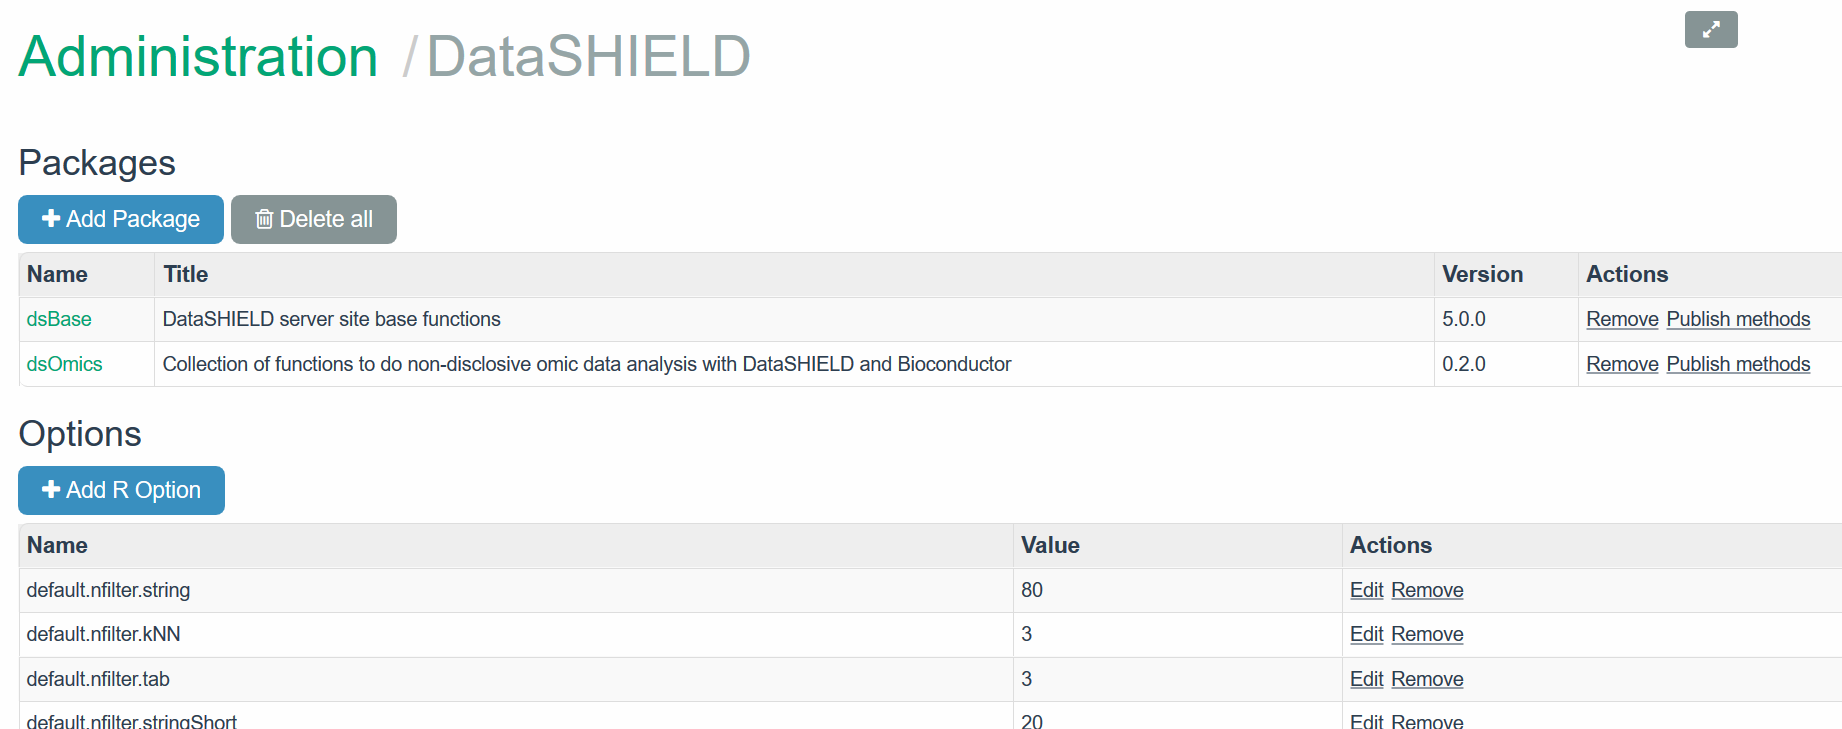
\includegraphics[width=25.58in]{fig/add_packages_opal} 

}

\caption{Installed packages in the test opal server}\label{fig:installPackagesOpal}
\end{figure}

The tab \textbf{+Add package} ca be used to install a new package. The
figure depicts how \texttt{dsOmics} was intalled into the opal server

\begin{figure}

{\centering 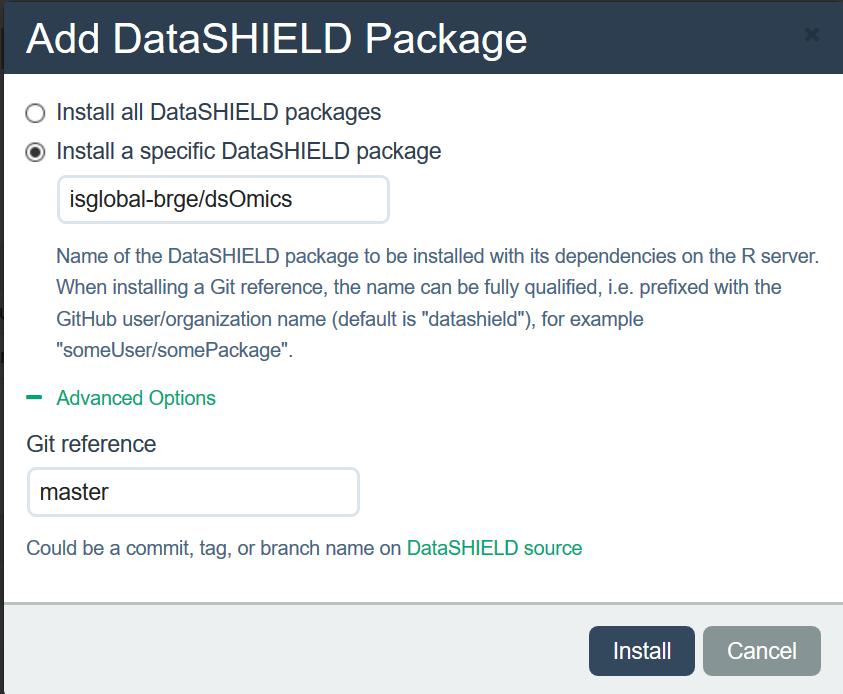
\includegraphics[width=0.9\linewidth]{fig/add_packages_opal_2} 

}

\caption{Description how `dsOmics` package was intalled into the test opal server}\label{fig:installPackagesOpal2}
\end{figure}

\hypertarget{required-r-packages-in-the-client-site-e.g.-local-machine}{%
\subsection{Required R Packages in the client site (e.g.~local
machine)}\label{required-r-packages-in-the-client-site-e.g.-local-machine}}

In order to use the functions contained within this package the
following R packages must be installed and loaded.

\begin{Shaded}
\begin{Highlighting}[]
\KeywordTok{library}\NormalTok{(resourcer)}
\KeywordTok{library}\NormalTok{(DSI)}
\KeywordTok{library}\NormalTok{(DSOpal)}
\KeywordTok{library}\NormalTok{(dsBaseClient)}
\KeywordTok{library}\NormalTok{(dsOmicsClient)}
\end{Highlighting}
\end{Shaded}

\textbf{Notes}:

\begin{itemize}
\tightlist
\item
  \texttt{dsOmicsClient} depends on \texttt{dsOmics} the
  \texttt{resourcer} package that can be installed by:
\end{itemize}

\begin{Shaded}
\begin{Highlighting}[]
\NormalTok{devtools}\OperatorTok{::}\KeywordTok{install\_github}\NormalTok{(}\StringTok{"obiba/resourcer"}\NormalTok{, }\DataTypeTok{dependencies =} \OtherTok{TRUE}\NormalTok{) }
\end{Highlighting}
\end{Shaded}

The other three packages can be installed by:

\begin{Shaded}
\begin{Highlighting}[]
\NormalTok{devtools}\OperatorTok{::}\KeywordTok{install\_github}\NormalTok{(}\StringTok{"datashield/DSI"}\NormalTok{, }\DataTypeTok{dependencies =} \OtherTok{TRUE}\NormalTok{)}
\NormalTok{devtools}\OperatorTok{::}\KeywordTok{install\_github}\NormalTok{(}\StringTok{"datashield/DSOpal"}\NormalTok{, }\DataTypeTok{dependencies =} \OtherTok{TRUE}\NormalTok{)}
\NormalTok{devtools}\OperatorTok{::}\KeywordTok{install\_github}\NormalTok{(}\StringTok{"datashield/dsBaseClient"}\NormalTok{, }\DataTypeTok{dependencies =} \OtherTok{TRUE}\NormalTok{)}
\NormalTok{devtools}\OperatorTok{::}\KeywordTok{install\_github}\NormalTok{(}\StringTok{"isglobal{-}brge/dsOmicsClient"}\NormalTok{, }\DataTypeTok{dependencies =} \OtherTok{TRUE}\NormalTok{)}
\end{Highlighting}
\end{Shaded}

\hypertarget{omics-data-analysis}{%
\section{Omics data analysis}\label{omics-data-analysis}}

\hypertarget{opal-and-resources}{%
\subsection{OPAL and resources}\label{opal-and-resources}}

The Figure \ref{fig:opalOmic} describes how omic associatin analyses are
performed using DataSHIELD client functions implemented in the
\texttt{\{r\ Githubpkg("isglobal-brge",\ "dsOmicsClient")} package.
Basically, data (omic and phenotypes/covariates) can be stored in
different sites (http, ssh, ASW W3, local, \ldots) and are managed with
Opal through the \texttt{\{r\ Githubpkg("obiba",\ "resourcer")} package
and their extensions implemented in
\texttt{\{r\ Githubpkg("isglobal-brge",\ "dsOmics")}.

\begin{figure}

{\centering 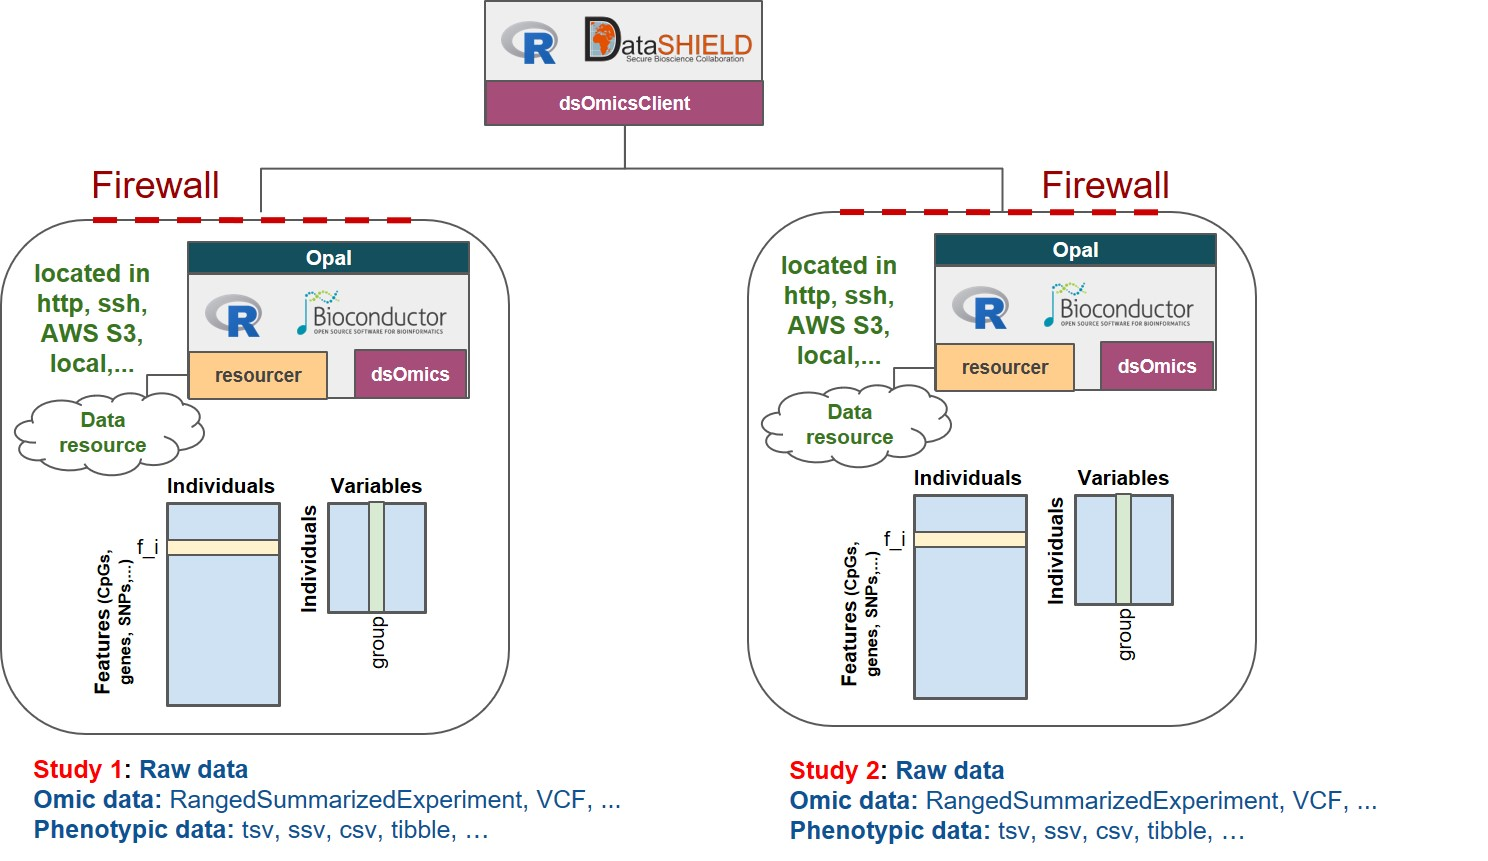
\includegraphics[width=1\linewidth]{fig/dsOmics_A} 

}

\caption{Non-disclosive omic data analysis with DataSHIELD and Bioconductor. The figure illustrates how the `resourcer` package is used to get access to omic data through the OPAL servers. Then DataSHIELD is used in the client side to perform non-disclosive data analyses.}\label{fig:opalOmic}
\end{figure}

Then, \texttt{dsOmicsClient} package allows different types of analyses:
pooled and meta-analysis.

The \textbf{pooled approach} (Figure \ref{fig:omicAnal1}) is recomended
when the user wants to analyze omic data from different sources and
obtain results as if the data were located in a single computer. It
should be noticed that this can be very time consuming when analyzing
multiple features since and that it cannot be recommended when data are
not properly harmonized (e.g.~gene expression normalized using different
methods, GWAS data having different platforms, \ldots). Also when it is
necesary to remove unwanted variability (for transcriptomic and
epigenomica analysis) or control for population stratification (for GWAS
analysis), this approach cannot be used since we need to develop methods
to compute surrogate variables (to remove unwanted variability) or PCAs
(to to address population stratification) in a non-disclosive way.

The \textbf{meta-analysis approach} Figure \ref{fig:omicAnal2} overcomes
the limitations raised when performing pooled analyses. First, the
computation issue is addressed by using scalable and fast methods to
perform data analysis at whole-genome level at each server. The
transcriptomic and epigenomic data analyses make use of the widely used
\emph{\href{https://bioconductor.org/packages/3.9/limma}{limma}} package
that uses \texttt{ExpressionSet} or \texttt{RangedSummarizedExperiment}
Bioc infrastructures to deal with omic and phenotypic (e.g covariates).
The genomic data are analyzed using
\emph{\href{https://bioconductor.org/packages/3.9/GWASTools}{GWASTools}}
and \emph{\href{https://bioconductor.org/packages/3.9/GENESIS}{GENESIS}}
that are designed to perform quality control (QC) and GWAS using GDS
infrastructure.

Next, we describe how both approaches are implemented:

\begin{itemize}
\tightlist
\item
  \textbf{Pooled approach:} Figure \ref{fig:omicAnal1} illustrate how
  this analysis is performed. This corresponds to generalized linear
  models (glm) on data from single or multiple sources. It makes use of
  \texttt{ds.glm()} function which is a DataSHIELD function that uses an
  approach that is mathematically equivalent to placing all
  individual-level data froma all sources in one central warehouse and
  analysing those data using the conventional \texttt{glm()} function in
  R. The user can select one (or multiple) features (i.e., genes,
  transcripts, CpGs, SNPs, \ldots)
\end{itemize}

\begin{figure}

{\centering 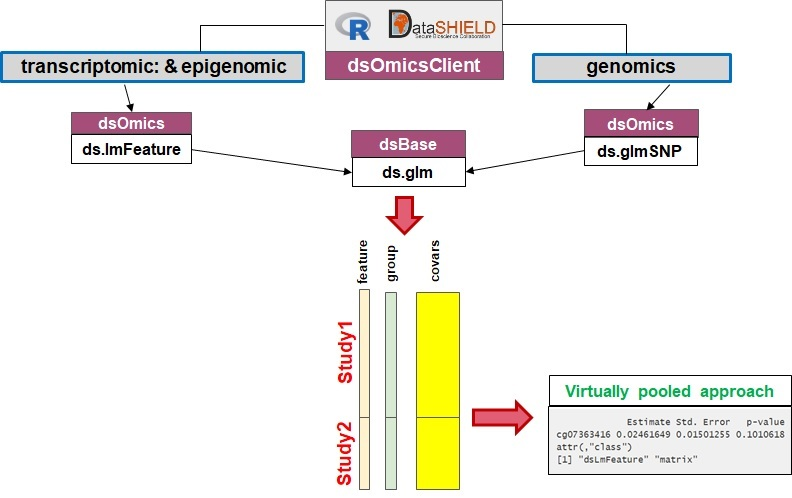
\includegraphics[width=1\linewidth]{fig/dsOmics_B} 

}

\caption{Non-disclosive omic data analysis with DataSHIELD and Bioconductor. The figure illustrates how to perform single pooled omic data analysis. The analyses are performed by using a generalized linear model (glm) on data from one or multiple sources. It makes use of `ds.glm()`, a DataSHIELD function, that uses an approach that is mathematically equivalent to placing all individual-level data froma all sources in one central warehouse and analysing those data using the conventional `glm()` function in R.}\label{fig:omicAnal1}
\end{figure}

\begin{itemize}
\tightlist
\item
  \textbf{Meta-analysis:} Figure \ref{fig:omicAnal2} illustrate how this
  analysis is performed. This corresponds to perform a genome-wide
  analysis at each server using functions that are specifically design
  to that purpose and that are scalable. Then the results of each server
  can be meta-analyzed unsing standard R package.
\end{itemize}

\begin{figure}

{\centering 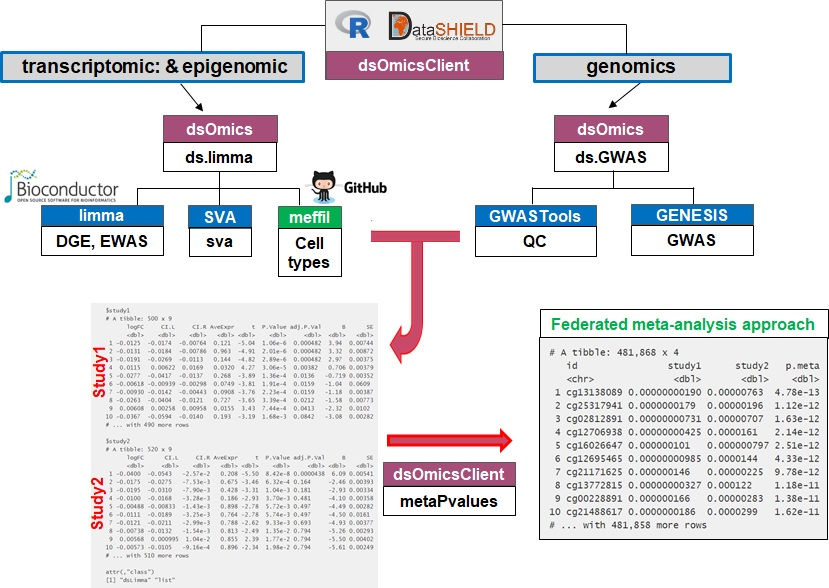
\includegraphics[width=10\linewidth]{fig/dsOmics_C} 

}

\caption{Non-disclosive omic data analysis with DataSHIELD and Bioconductor. The figure illustrates how to perform anlyses at genome-wide level from one or multiple sources. It runs standard Bioconductor functions at each server independently to speed up the analyses and in the case of having multiple sources, results can be meta-analyzed uning standar R functions.}\label{fig:omicAnal2}
\end{figure}

\hypertarget{analysis-of-methylation-data}{%
\section{Analysis of methylation
data}\label{analysis-of-methylation-data}}

Here we illustrate how to analyze methylation data stored as an
\texttt{ExpressionSet}. Epigenomic data can also be encapsulated as a
\texttt{GenomicRatioSet}. The analyses for this type of objects can be
performed as here is illustrated for \texttt{ExpressionSet} since the
functions automatically detects the type of object passed through the
main functions.

Figure \ref{fig:testResources} shows that our test opal server contains
two data sets (GSE80970.Rdata and GSE66351.Rdata) having information on
DNA methylation profiling. Both are R data files containing an object of
\texttt{ExpressionSet} class. Data corresponds to CpGs beta values
measured in the superior temporal gyrus and prefrontal cortex brain
regions of patients with Alzheimer's. These data have been downloaded
from GEO (\url{https://www.ncbi.nlm.nih.gov/geo/}) using the GEO
accession numbers GSE80970 and GSE66351, respectively. Researchers who
are not familiar with \texttt{ExpressionSet}s or for those who have data
in other formats, this page
(\url{https://kasperdanielhansen.github.io/genbioconductor/html/ExpressionSet.html})
can be used as a good starting point to undersatand how methylation data
can be encapsulated in a \texttt{ExpressionSet}.

\begin{itemize}
\tightlist
\item
  \textbf{indicate that CpG must contain beta values and not M values}
\item
  \textbf{this can be checked and computed in the servers}
\end{itemize}

First, we start by login and assigning resources to DataSHIELD

\begin{Shaded}
\begin{Highlighting}[]
\NormalTok{builder <{-}}\StringTok{ }\NormalTok{DSI}\OperatorTok{::}\KeywordTok{newDSLoginBuilder}\NormalTok{()}
\NormalTok{builder}\OperatorTok{$}\KeywordTok{append}\NormalTok{(}\DataTypeTok{server =} \StringTok{"study1"}\NormalTok{, }\DataTypeTok{url =} \StringTok{"https://opal{-}test.obiba.org"}\NormalTok{, }
               \DataTypeTok{user =} \StringTok{"dsuser"}\NormalTok{, }\DataTypeTok{password =} \StringTok{"password"}\NormalTok{, }
               \DataTypeTok{resource =} \StringTok{"test.GSE66351"}\NormalTok{, }\DataTypeTok{driver =} \StringTok{"OpalDriver"}\NormalTok{)}
\NormalTok{builder}\OperatorTok{$}\KeywordTok{append}\NormalTok{(}\DataTypeTok{server =} \StringTok{"study2"}\NormalTok{, }\DataTypeTok{url =} \StringTok{"https://opal{-}test.obiba.org"}\NormalTok{, }
               \DataTypeTok{user =} \StringTok{"dsuser"}\NormalTok{, }\DataTypeTok{password =} \StringTok{"password"}\NormalTok{, }
               \DataTypeTok{resource =} \StringTok{"test.GSE80970"}\NormalTok{, }\DataTypeTok{driver =} \StringTok{"OpalDriver"}\NormalTok{)}

\NormalTok{logindata <{-}}\StringTok{ }\NormalTok{builder}\OperatorTok{$}\KeywordTok{build}\NormalTok{()}

\NormalTok{conns <{-}}\StringTok{ }\NormalTok{DSI}\OperatorTok{::}\KeywordTok{datashield.login}\NormalTok{(}\DataTypeTok{logins =}\NormalTok{ logindata, }\DataTypeTok{assign =} \OtherTok{TRUE}\NormalTok{, }
                               \DataTypeTok{symbol =} \StringTok{"res"}\NormalTok{)}
\end{Highlighting}
\end{Shaded}

After that, we check whether the opal server has the assigned resources.
This can be performed by using a function from \texttt{dsBaseClient}
package.

\begin{Shaded}
\begin{Highlighting}[]
\KeywordTok{ds.ls}\NormalTok{()}
\end{Highlighting}
\end{Shaded}

\begin{verbatim}
$study1
[1] "res"

$study2
[1] "res"
\end{verbatim}

The \texttt{ExpressionSet} object (accessed by the resource client)
could be coerced to a data frame by

\begin{Shaded}
\begin{Highlighting}[]
\KeywordTok{datashield.assign.expr}\NormalTok{(conns, }\DataTypeTok{symbol =} \StringTok{"methyl\_df"}\NormalTok{, }
                       \DataTypeTok{expr =} \KeywordTok{quote}\NormalTok{(}\KeywordTok{as.resource.data.frame}\NormalTok{(res)))}
\KeywordTok{ds.class}\NormalTok{(}\StringTok{"methyl\_df"}\NormalTok{)}
\end{Highlighting}
\end{Shaded}

\begin{verbatim}
$study1
[1] "data.frame"

$study2
[1] "data.frame"
\end{verbatim}

The coercion creates a data frame with CpGs and covariables in columns.
We do not recomment to work with data frames for omic data since
Bioconductor has efficient classes to deal with this type of data. We
just illustrate that this coercion is possible and then DataSHIELD
functions can be used to perform different statistical analyses. For
instance, a data frame can be inspected, using \texttt{dsBaseClient}
functions

\begin{Shaded}
\begin{Highlighting}[]
\KeywordTok{ds.summary}\NormalTok{(}\StringTok{"methyl\_df$casecon"}\NormalTok{)}
\end{Highlighting}
\end{Shaded}

\begin{verbatim}
$study1
$study1$class
[1] "character"

$study1$length
[1] 190


$study2
$study2$class
[1] "character"

$study2$length
[1] 286
\end{verbatim}

\begin{Shaded}
\begin{Highlighting}[]
\KeywordTok{ds.summary}\NormalTok{(}\StringTok{"methyl\_df$cg07363416"}\NormalTok{)}
\end{Highlighting}
\end{Shaded}

\begin{verbatim}
$study1
$study1$class
[1] "numeric"

$study1$length
[1] 190

$study1$`quantiles & mean`
      5%      10%      25%      50%      75%      90%      95%     Mean 
0.000000 0.000000 0.000000 0.000000 0.131490 0.434133 0.505164 0.101368 


$study2
$study2$class
[1] "numeric"

$study2$length
[1] 286

$study2$`quantiles & mean`
       5%       10%       25%       50%       75%       90%       95% 
0.1528750 0.1614350 0.1771200 0.4307500 0.4624325 0.4803350 0.4947300 
     Mean 
0.3471427 
\end{verbatim}

Another example is that we can fit a glm model in the multiple studies
using an approach that is similar to analyze pooled data

\begin{Shaded}
\begin{Highlighting}[]
\KeywordTok{ds.glm}\NormalTok{(cg07363416 }\OperatorTok{\textasciitilde{}}\StringTok{ }\NormalTok{casecon }\OperatorTok{+}\StringTok{ }\NormalTok{Sex, }\DataTypeTok{data=}\StringTok{"methyl\_df"}\NormalTok{,}
       \DataTypeTok{family=}\StringTok{"binomial"}\NormalTok{)}
\end{Highlighting}
\end{Shaded}

\begin{verbatim}
$Nvalid
[1] 476

$Nmissing
[1] 0

$Ntotal
[1] 476

$disclosure.risk
       RISK OF DISCLOSURE
study1                  0
study2                  0

$errorMessage
       ERROR MESSAGES
study1 "No errors"   
study2 "No errors"   

$nsubs
[1] 476

$iter
[1] 6

$family

Family: binomial 
Link function: logit 


$formula
[1] "cg07363416 ~ casecon + Sex"

$coefficients
              Estimate Std. Error    z-value      p-value low0.95CI.LP
(Intercept) -0.6912109  0.1529100 -4.5203776 6.172942e-06   -0.9909090
caseconCTRL  0.1422289  0.2265482  0.6278085 5.301294e-01   -0.3017974
SexM        -1.4665544  0.2644814 -5.5450194 2.939215e-08   -1.9849284
            high0.95CI.LP      P_OR low0.95CI.P_OR high0.95CI.P_OR
(Intercept)    -0.3915128 0.3337637      0.2707326       0.4033532
caseconCTRL     0.5862552 1.1528405      0.7394879       1.7972455
SexM           -0.9481804 0.2307191      0.1373905       0.3874454

$dev
[1] 86.82906

$df
[1] 473

$output.information
[1] "SEE TOP OF OUTPUT FOR INFORMATION ON MISSING DATA AND ERROR MESSAGES"
\end{verbatim}

As previously mention it is prefered to directly extract the R object as
Bioconductor's \texttt{ExpressionSet}. This can be performed since
DataSHIELD configuration allows \texttt{as.resource.object()} assignment
function.

\begin{Shaded}
\begin{Highlighting}[]
\KeywordTok{datashield.assign.expr}\NormalTok{(conns, }\DataTypeTok{symbol =} \StringTok{"methy"}\NormalTok{, }
                       \DataTypeTok{expr =} \KeywordTok{quote}\NormalTok{(}\KeywordTok{as.resource.object}\NormalTok{(res)))}
\KeywordTok{ds.class}\NormalTok{(}\StringTok{"methy"}\NormalTok{)}
\end{Highlighting}
\end{Shaded}

\begin{verbatim}
$study1
[1] "ExpressionSet"
attr(,"package")
[1] "Biobase"

$study2
[1] "ExpressionSet"
attr(,"package")
[1] "Biobase"
\end{verbatim}

Then, some Bioconductor-type functions can be use to get non-disclosive
information of \texttt{ExpressionSet}s at each server from the client
using similar functions as those defined in \texttt{dsBaseClient}. For
example, feature names can be seen by

\begin{Shaded}
\begin{Highlighting}[]
\NormalTok{fn <{-}}\StringTok{ }\KeywordTok{ds.featureNames}\NormalTok{(}\StringTok{"methy"}\NormalTok{)}
\KeywordTok{lapply}\NormalTok{(fn, head)}
\end{Highlighting}
\end{Shaded}

\begin{verbatim}
$study1
[1] "cg21477232" "cg15065877" "cg22631350" "cg13376768" "cg21915026"
[6] "cg23203918"

$study2
[1] "cg21477232" "cg15065877" "cg22631350" "cg13376768" "cg21915026"
[6] "cg23203918"
\end{verbatim}

Experimental phenotypes variables can be obtained by

\begin{Shaded}
\begin{Highlighting}[]
\KeywordTok{ds.varLabels}\NormalTok{(}\StringTok{"methy"}\NormalTok{)}
\end{Highlighting}
\end{Shaded}

\begin{verbatim}
$study1
 [1] "title"                   "geo_accession"          
 [3] "status"                  "submission_date"        
 [5] "last_update_date"        "type"                   
 [7] "channel_count"           "source_name_ch1"        
 [9] "organism_ch1"            "characteristics_ch1"    
[11] "characteristics_ch1.1"   "characteristics_ch1.2"  
[13] "characteristics_ch1.3"   "characteristics_ch1.4"  
[15] "characteristics_ch1.5"   "characteristics_ch1.6"  
[17] "characteristics_ch1.7"   "characteristics_ch1.8"  
[19] "molecule_ch1"            "extract_protocol_ch1"   
[21] "label_ch1"               "label_protocol_ch1"     
[23] "taxid_ch1"               "hyb_protocol"           
[25] "scan_protocol"           "description"            
[27] "data_processing"         "platform_id"            
[29] "contact_name"            "contact_email"          
[31] "contact_phone"           "contact_laboratory"     
[33] "contact_institute"       "contact_address"        
[35] "contact_city"            "contact_zip/postal_code"
[37] "contact_country"         "supplementary_file"     
[39] "supplementary_file.1"    "data_row_count"         
[41] "age"                     "braak_stage:ch1"        
[43] "brain_region:ch1"        "cell type:ch1"          
[45] "casecon"                 "donor_id:ch1"           
[47] "sentrix_id:ch1"          "sentrix_position:ch1"   
[49] "Sex"                    

$study2
 [1] "title"                   "geo_accession"          
 [3] "status"                  "submission_date"        
 [5] "last_update_date"        "type"                   
 [7] "channel_count"           "source_name_ch1"        
 [9] "organism_ch1"            "characteristics_ch1"    
[11] "characteristics_ch1.1"   "characteristics_ch1.2"  
[13] "characteristics_ch1.3"   "characteristics_ch1.4"  
[15] "characteristics_ch1.5"   "characteristics_ch1.6"  
[17] "molecule_ch1"            "extract_protocol_ch1"   
[19] "label_ch1"               "label_protocol_ch1"     
[21] "taxid_ch1"               "hyb_protocol"           
[23] "scan_protocol"           "description"            
[25] "description.1"           "data_processing"        
[27] "platform_id"             "contact_name"           
[29] "contact_email"           "contact_department"     
[31] "contact_institute"       "contact_address"        
[33] "contact_city"            "contact_state"          
[35] "contact_zip/postal_code" "contact_country"        
[37] "supplementary_file"      "data_row_count"         
[39] "age"                     "braak stage:ch1"        
[41] "casecon"                 "donor id:ch1"           
[43] "Sex"                     "sentrix id:ch1"         
[45] "tissue:ch1"             

attr(,"class")
[1] "dsvarLabels" "list"       
\end{verbatim}

\hypertarget{single-cpg-analysis}{%
\subsection{Single CpG analysis}\label{single-cpg-analysis}}

Once the methylation data have been loaded into the opal server, we can
perform different type of analyses using \texttt{dsOmicsClient}. Let us
start by illustrating how to analyze a single CpG from two studies by
using an approach that is mathematically equivalent to placing all
individual-level.

\begin{Shaded}
\begin{Highlighting}[]
\NormalTok{ans <{-}}\StringTok{ }\KeywordTok{ds.lmFeature}\NormalTok{(}\DataTypeTok{feature=}\StringTok{"cg07363416"}\NormalTok{, }
                    \DataTypeTok{model=}\NormalTok{casecon}\OperatorTok{\textasciitilde{}}\NormalTok{Sex, }
                    \DataTypeTok{eSet=}\StringTok{"methy"}\NormalTok{,}
                    \DataTypeTok{datasources=}\NormalTok{conns)}
\NormalTok{ans}
\end{Highlighting}
\end{Shaded}

\begin{verbatim}
             Estimate Std. Error   p-value
cg07363416 0.02461649 0.01501255 0.1010618
attr(,"class")
[1] "dsLmFeature" "matrix"     
\end{verbatim}

\hypertarget{genome-wide-cpg-analysis}{%
\subsection{Genome-wide CpG analysis}\label{genome-wide-cpg-analysis}}

The same analysis can be performed for all features (e.g.~CpGs) just
avoiding the \{\tt feature\} argument. This process can be parallelized
using \texttt{mclapply} function from \texttt{multicore} package.

\begin{Shaded}
\begin{Highlighting}[]
\NormalTok{ans <{-}}\StringTok{ }\KeywordTok{ds.lmFeature}\NormalTok{(}\DataTypeTok{model =}\NormalTok{ casecon}\OperatorTok{\textasciitilde{}}\NormalTok{Sex, }
                    \DataTypeTok{eSet =} \StringTok{"methy"}\NormalTok{,}
                    \DataTypeTok{datasources =}\NormalTok{ conns,}
                    \DataTypeTok{mc.cores =} \DecValTok{20}\NormalTok{)}
\end{Highlighting}
\end{Shaded}

We can create a QQ-plot by using the generic function \texttt{plot}
\ldots.

This method can be very time consiming since the function repeteadly
calls the DataSHIELD function \texttt{ds.glm()}. We can adopt another
strategy that is to run a glm of each feature independently at each
study using \texttt{limma} package which is really fast.

\begin{Shaded}
\begin{Highlighting}[]
\NormalTok{ans.limma <{-}}\StringTok{ }\KeywordTok{ds.limma}\NormalTok{(}\DataTypeTok{model =} \OperatorTok{\textasciitilde{}}\StringTok{ }\NormalTok{casecon }\OperatorTok{+}\StringTok{ }\NormalTok{Sex,}
                      \DataTypeTok{Set =} \StringTok{"methy"}\NormalTok{, }
                      \DataTypeTok{datasources =}\NormalTok{ conns)}
\NormalTok{ans.limma}
\end{Highlighting}
\end{Shaded}

\begin{verbatim}
$study1
# A tibble: 500 x 9
      logFC     CI.L     CI.R AveExpr     t P.Value adj.P.Val      B
      <dbl>    <dbl>    <dbl>   <dbl> <dbl>   <dbl>     <dbl>  <dbl>
 1 -0.0125  -0.0174  -0.00764  0.121  -5.04 1.06e-6  0.000482  3.94 
 2 -0.0131  -0.0184  -0.00786  0.963  -4.91 2.01e-6  0.000482  3.32 
 3 -0.0191  -0.0269  -0.0113   0.144  -4.82 2.89e-6  0.000482  2.97 
 4  0.0115   0.00622  0.0169   0.0320  4.27 3.06e-5  0.00382   0.706
 5 -0.0277  -0.0417  -0.0137   0.268  -3.89 1.36e-4  0.0136   -0.719
 6 -0.00618 -0.00939 -0.00298  0.0749 -3.81 1.91e-4  0.0159   -1.04 
 7 -0.00930 -0.0142  -0.00443  0.0908 -3.76 2.23e-4  0.0159   -1.18 
 8 -0.0263  -0.0404  -0.0121   0.727  -3.65 3.39e-4  0.0212   -1.58 
 9  0.00608  0.00258  0.00958  0.0155  3.43 7.44e-4  0.0413   -2.32 
10 -0.0367  -0.0594  -0.0140   0.193  -3.19 1.68e-3  0.0842   -3.08 
# ... with 490 more rows, and 1 more variable: SE <dbl>

$study2
# A tibble: 520 x 9
      logFC     CI.L     CI.R AveExpr     t P.Value adj.P.Val     B      SE
      <dbl>    <dbl>    <dbl>   <dbl> <dbl>   <dbl>     <dbl> <dbl>   <dbl>
 1 -0.0400  -5.43e-2 -2.57e-2   0.208 -5.50 8.42e-8 0.0000438  6.09 0.00541
 2 -0.0175  -2.75e-2 -7.53e-3   0.675 -3.46 6.32e-4 0.164     -2.46 0.00393
 3 -0.0195  -3.10e-2 -7.90e-3   0.428 -3.31 1.04e-3 0.181     -2.93 0.00334
 4 -0.0100  -1.68e-2 -3.28e-3   0.186 -2.93 3.70e-3 0.481     -4.10 0.00358
 5 -0.00488 -8.33e-3 -1.43e-3   0.898 -2.78 5.72e-3 0.497     -4.49 0.00282
 6 -0.0111  -1.89e-2 -3.25e-3   0.764 -2.78 5.74e-3 0.497     -4.50 0.0161 
 7 -0.0121  -2.11e-2 -2.99e-3   0.788 -2.62 9.33e-3 0.693     -4.93 0.00377
 8 -0.00738 -1.32e-2 -1.54e-3   0.813 -2.49 1.35e-2 0.794     -5.26 0.00293
 9  0.00568  9.95e-4  1.04e-2   0.855  2.39 1.77e-2 0.794     -5.50 0.00402
10 -0.00573 -1.05e-2 -9.16e-4   0.896 -2.34 1.98e-2 0.794     -5.61 0.00249
# ... with 510 more rows

attr(,"class")
[1] "dsLimma" "list"   
\end{verbatim}

The annotation can be added by \ldots{}

Then, the results can be combined by \ldots.

\hypertarget{adjusting-for-cell-type}{%
\subsection{Adjusting for cell-type}\label{adjusting-for-cell-type}}

The vast majority of studies on DNA methylation are based on blood
samples. This required to adjust for variability in cell-type mixture
proportions. There are several method to address this issue. Here we
adopt the methods proposed in the \texttt{meffill} package by using
\texttt{meffil.estimate.cell.counts.from.betas()} function.
\texttt{dsOmicsClient} can fit a model adjusted for cell-type
composition by setting the argument \texttt{cellCountsAdjust=TRUE}.

\begin{itemize}
\tightlist
\item
  \textbf{implementation description to be provided}
\item
  \textbf{get error if required CpGs are not available}
\end{itemize}

\begin{Shaded}
\begin{Highlighting}[]
\NormalTok{ans.cell <{-}}\StringTok{ }\KeywordTok{ds.lmFeature}\NormalTok{(}\DataTypeTok{feature =} \StringTok{"cg07363416"}\NormalTok{, }
                    \DataTypeTok{model =}\NormalTok{ casecon }\OperatorTok{\textasciitilde{}}\StringTok{ }\NormalTok{Sex, }
                    \DataTypeTok{eSet =} \StringTok{"methy"}\NormalTok{, }
                    \DataTypeTok{cellCountsAdjust =} \OtherTok{TRUE}\NormalTok{,}
                    \DataTypeTok{datasources =}\NormalTok{ conns)}
\end{Highlighting}
\end{Shaded}

\begin{verbatim}
Error in ds.lmFeature(feature = "cg07363416", model = casecon ~ Sex, eSet = "methy", : There is any problem with cell-type estimation in at least one study
\end{verbatim}

\hypertarget{adjusting-for-surrogate-variables}{%
\subsection{Adjusting for Surrogate
Variables}\label{adjusting-for-surrogate-variables}}

The vast majority of omic studies required to control for unwanted
variability. The surrogate variable analysis (SVA) can address this
issue by estimating some hidden covariates that capture differences
across individuals due to some artifacts such as batch effects or sample
quality sam among others. The method is implemented in
\emph{\href{https://bioconductor.org/packages/3.9/SVA}{SVA}} package.

Performing this type of analysis using \texttt{ds.lmFeature} function is
not allowed since estimating SVA would require to implement a
non-disclosive method that computes SVA from the different servers. This
will be a future topic of \texttt{dsOmicsClient}. NOTE that, estimating
SVA separately at each server would not be a good idea since the aim of
SVA is to capture differences mainly due to experiemental issues amogn
ALL individuals. What we can do instead is to use \texttt{ds.limma} and
perform the analyses adjusted for SVA at each study. Then, data can be
combined using \ldots{}

\begin{Shaded}
\begin{Highlighting}[]
\NormalTok{ans.sva <{-}}\StringTok{ }\KeywordTok{ds.limma}\NormalTok{(}\DataTypeTok{model =}\NormalTok{ casecon }\OperatorTok{\textasciitilde{}}\StringTok{ }\NormalTok{Sex, }
                    \DataTypeTok{Set =} \StringTok{"methy"}\NormalTok{,}
                    \DataTypeTok{sva =} \OtherTok{TRUE}\NormalTok{)}
\end{Highlighting}
\end{Shaded}

\begin{verbatim}
Error: Command 'limmaDS(methy,"casecon","Sex",1,TRUE,NULL)' failed on 'study2': Error while evaluating 'dsOmics::limmaDS(methy, "casecon", "Sex", 1, TRUE, NULL)' -> Error in do.call(.Call, args = dot_call_args) : 
  TridiagEigen: eigen decomposition failed
\end{verbatim}

The DataSHIELD session must by closed by:

\begin{Shaded}
\begin{Highlighting}[]
\KeywordTok{datashield.logout}\NormalTok{(conns)}
\end{Highlighting}
\end{Shaded}

\hypertarget{analysis-of-transcriptomic-data}{%
\section{Analysis of transcriptomic
data}\label{analysis-of-transcriptomic-data}}

The analysis of gene expression can also be performed using
\emph{\href{https://bioconductor.org/packages/3.9/limma}{limma}}
package. In that case, it is not recommended to use the function
\texttt{ds.lmFeature} since gene expression can have different range of
values accross studies (this is different from methylation where CpG
data is measured in the range 0-1). However, if data of each study have
been harmonized this function can also be used to get results as if it
had been used a pooled data analysis.

Let us illustrate how to perform transcriptomic data analysis from
\href{https://www.cancer.gov/about-nci/organization/ccg/research/structural-genomics/tcga}{TCGA
project}. We have uploaded to the opal server a resource called
\texttt{tcga\_liver} whose URL is
\url{http://duffel.rail.bio/recount/TCGA/rse_gene_liver.Rdata} which is
available through the
\href{https://jhubiostatistics.shinyapps.io/recount/}{recount project}.
This resource contains the \texttt{RangeSummarizedExperiment} with the
RNAseq profiling of liver cancer data from TCGA. Next, we illustrate how
a differential expression analysis to compare RNAseq profiling of women
vs men (variable \texttt{gdc\_cases.demographic.gender}).

Let us start by creating the connection to the opal server:

\begin{Shaded}
\begin{Highlighting}[]
\NormalTok{builder <{-}}\StringTok{ }\KeywordTok{newDSLoginBuilder}\NormalTok{()}
\NormalTok{builder}\OperatorTok{$}\KeywordTok{append}\NormalTok{(}\DataTypeTok{server =} \StringTok{"study1"}\NormalTok{, }\DataTypeTok{url =} \StringTok{"https://opal{-}test.obiba.org"}\NormalTok{, }
               \DataTypeTok{user =} \StringTok{"dsuser"}\NormalTok{, }\DataTypeTok{password =} \StringTok{"password"}\NormalTok{, }
               \DataTypeTok{resource =} \StringTok{"test.tcga\_liver"}\NormalTok{, }\DataTypeTok{driver =} \StringTok{"OpalDriver"}\NormalTok{)}

\NormalTok{logindata <{-}}\StringTok{ }\NormalTok{builder}\OperatorTok{$}\KeywordTok{build}\NormalTok{()}

\NormalTok{conns <{-}}\StringTok{ }\KeywordTok{datashield.login}\NormalTok{(}\DataTypeTok{logins =}\NormalTok{ logindata, }\DataTypeTok{assign =} \OtherTok{TRUE}\NormalTok{, }
                          \DataTypeTok{symbol =} \StringTok{"res"}\NormalTok{)}
\end{Highlighting}
\end{Shaded}

Then, let us coerce the resource to a
\texttt{RangedSummarizedExperiment} which is the type of object that are
available in the
\href{https://jhubiostatistics.shinyapps.io/recount/}{recount project}.

\begin{Shaded}
\begin{Highlighting}[]
\KeywordTok{datashield.assign.expr}\NormalTok{(conns, }\DataTypeTok{symbol =} \StringTok{"rse"}\NormalTok{, }
                       \DataTypeTok{expr =} \KeywordTok{quote}\NormalTok{(}\KeywordTok{as.resource.object}\NormalTok{(res)))}
\KeywordTok{ds.class}\NormalTok{(}\StringTok{"rse"}\NormalTok{)}
\end{Highlighting}
\end{Shaded}

\begin{verbatim}
$study1
[1] "RangedSummarizedExperiment"
attr(,"package")
[1] "SummarizedExperiment"
\end{verbatim}

The number of features and samples can be inspected by

\begin{Shaded}
\begin{Highlighting}[]
\KeywordTok{ds.dim}\NormalTok{(}\StringTok{"rse"}\NormalTok{)}
\end{Highlighting}
\end{Shaded}

\begin{verbatim}
$`dimensions of rse in study1`
[1] 58037   424

$`dimensions of rse in combined studies`
[1] 58037   424
\end{verbatim}

And the names of the features using the same function used in the case
of analyzing an \texttt{ExpressionSet}

\begin{Shaded}
\begin{Highlighting}[]
\NormalTok{name.features <{-}}\StringTok{ }\KeywordTok{ds.featureNames}\NormalTok{(}\StringTok{"rse"}\NormalTok{)}
\KeywordTok{lapply}\NormalTok{(name.features, head)}
\end{Highlighting}
\end{Shaded}

\begin{verbatim}
$study1
[1] "ENSG00000000003.14" "ENSG00000000005.5"  "ENSG00000000419.12"
[4] "ENSG00000000457.13" "ENSG00000000460.16" "ENSG00000000938.12"
\end{verbatim}

Also the covariate names can be inspected by

\begin{Shaded}
\begin{Highlighting}[]
\NormalTok{name.vars <{-}}\StringTok{ }\KeywordTok{ds.featureData}\NormalTok{(}\StringTok{"rse"}\NormalTok{)}
\KeywordTok{lapply}\NormalTok{(name.vars, head, }\DataTypeTok{n=}\DecValTok{15}\NormalTok{)}
\end{Highlighting}
\end{Shaded}

\begin{verbatim}
$study1
 [1] "project"                                       
 [2] "sample"                                        
 [3] "experiment"                                    
 [4] "run"                                           
 [5] "read_count_as_reported_by_sra"                 
 [6] "reads_downloaded"                              
 [7] "proportion_of_reads_reported_by_sra_downloaded"
 [8] "paired_end"                                    
 [9] "sra_misreported_paired_end"                    
[10] "mapped_read_count"                             
[11] "auc"                                           
[12] "sharq_beta_tissue"                             
[13] "sharq_beta_cell_type"                          
[14] "biosample_submission_date"                     
[15] "biosample_publication_date"                    
\end{verbatim}

We can visualize the levels of the variable having gender information

\begin{Shaded}
\begin{Highlighting}[]
\KeywordTok{ds.table1D}\NormalTok{(}\StringTok{"rse$gdc\_cases.demographic.gender"}\NormalTok{)}
\end{Highlighting}
\end{Shaded}

\begin{verbatim}
$counts
       rse$gdc_cases.demographic.gender
female                              143
male                                281
Total                               424

$percentages
       rse$gdc_cases.demographic.gender
female                            33.73
male                              66.27
Total                            100.00

$validity
[1] "All tables are valid!"
\end{verbatim}

The differential expression analysis is then performed by:

\begin{Shaded}
\begin{Highlighting}[]
\NormalTok{ans.gender <{-}}\StringTok{ }\KeywordTok{ds.limma}\NormalTok{(}\DataTypeTok{model =}  \OperatorTok{\textasciitilde{}}\StringTok{ }\NormalTok{gdc\_cases.demographic.gender, }
                   \DataTypeTok{Set =} \StringTok{"rse"}\NormalTok{, }\DataTypeTok{type.data =} \StringTok{"RNAseq"}\NormalTok{, }
                   \DataTypeTok{sva =} \OtherTok{FALSE}\NormalTok{)}
\end{Highlighting}
\end{Shaded}

Notice that in that case we have set
\texttt{type.data=\textquotesingle{}RNAseq\textquotesingle{}} since our
data are counts obtained from a NGS experiment. By indicating so, the
differential analysis is performed by using \texttt{voom} +
\texttt{limma} implemented in the
\emph{\href{https://bioconductor.org/packages/3.9/MEAL}{MEAL}} package.

As usual, we close the DataSHIELD session by:

\begin{Shaded}
\begin{Highlighting}[]
\KeywordTok{datashield.logout}\NormalTok{(conns)}
\end{Highlighting}
\end{Shaded}

\hypertarget{analysis-of-snp-array-data}{%
\section{Analysis of SNP array data}\label{analysis-of-snp-array-data}}

\hypertarget{extension-of-the-resources-to-a-vcf-file}{%
\subsection{Extension of the resources to a VCF
file}\label{extension-of-the-resources-to-a-vcf-file}}

Genomic data can be stored in different formats.
\href{http://zzz.bwh.harvard.edu/plink/}{PLINK} and
\href{https://www.internationalgenome.org/wiki/Analysis/vcf4.0/}{VCF}
files are commonly used in genetic epidemiology studies. In order to
deal with this type of data, we have extended the resources available at
the \emph{\href{https://github.com/obiba}{resourcer}} package to VCF
files. \textbf{NOTE}: PLINK files can be translated into VCF files using
different pipelines. In R you can use
\emph{\href{https://bioconductor.org/packages/3.9/SeqArray}{SeqArray}}
to get VCF files.

We use the Genomic Data Storage (GDS) format which efficiently manage
VCF files into the R environment. This extension requires to create a
Client and a Resolver function that are located into the
\emph{\href{https://bioconductor.org/packages/3.9/dsOmics}{dsOmics}}
package. The client function uses \texttt{snpgdsVCF2GDS} function
implemented in
\emph{\href{https://bioconductor.org/packages/3.9/SNPrelate}{SNPrelate}}
to coerce the VCF file to a GDS object. Then the GDS object is loaded
into R as an object of class \texttt{GdsGenotypeReader} from
\emph{\href{https://bioconductor.org/packages/3.9/GWASTools}{GWASTools}}
package that facilitates downstream analyses.

The opal API server allows to incorporte this new type of resource as
illustrated in the figure:

\begin{figure}

{\centering 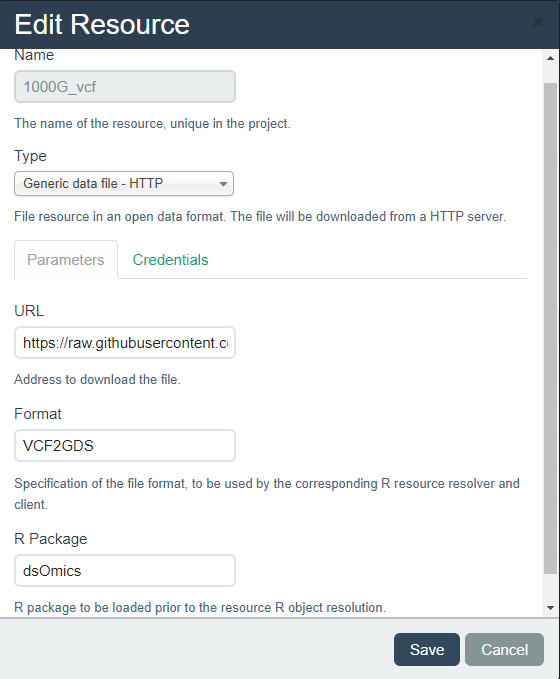
\includegraphics[width=1\linewidth]{fig/opal_resource_VCF} 

}

\caption{Description of how a VCF file can be added to the opal resources}\label{fig:resourceVCF}
\end{figure}

It is important to notice that the URL should contain the tag
\texttt{method=biallelic.only\&snpfirstdim=TRUE} since these are
required parameters of \texttt{snpgdsVCF2GDS} function. This is an
example:

\begin{verbatim}
https://raw.githubusercontent.com/isglobal-brge/scoreInvHap/master/inst/extdata/example.vcf?method=biallelic.only&snpfirstdim=TRUE
\end{verbatim}

In that case we indicate that only biallelic SNPs are considered
(`method=biallelic.only') and that genotypes are stored in the
individual-major mode, (i.e, list all SNPs for the first individual, and
then list all SNPs for the second individual, etc) (`snpfirstdim=TRUE').

\hypertarget{assigning-the-resources-vcf-file-and-to-the-opal-server}{%
\subsection{Assigning the resources (VCF file and ) to the OPAL
server}\label{assigning-the-resources-vcf-file-and-to-the-opal-server}}

We are using a GWAS example described in \ldots\ldots{}

We first start by preparing login data

\begin{Shaded}
\begin{Highlighting}[]
\NormalTok{builder <{-}}\StringTok{ }\KeywordTok{newDSLoginBuilder}\NormalTok{()}
\NormalTok{builder}\OperatorTok{$}\KeywordTok{append}\NormalTok{(}\DataTypeTok{server =} \StringTok{"study1"}\NormalTok{, }\DataTypeTok{url =} \StringTok{"https://opal{-}test.obiba.org"}\NormalTok{,}
               \DataTypeTok{user =} \StringTok{"dsuser"}\NormalTok{, }\DataTypeTok{password =} \StringTok{"password"}\NormalTok{,}
               \DataTypeTok{resource =} \StringTok{"test.obesity\_vcf"}\NormalTok{, }\DataTypeTok{driver =} \StringTok{"OpalDriver"}\NormalTok{)}
\NormalTok{logindata <{-}}\StringTok{ }\NormalTok{builder}\OperatorTok{$}\KeywordTok{build}\NormalTok{()}

\NormalTok{conns <{-}}\StringTok{ }\KeywordTok{datashield.login}\NormalTok{(}\DataTypeTok{logins =}\NormalTok{ logindata, }\DataTypeTok{assign =} \OtherTok{TRUE}\NormalTok{,}
                          \DataTypeTok{symbol =} \StringTok{"res"}\NormalTok{)}
\end{Highlighting}
\end{Shaded}

In this case we have to assign to different resources. One for the VCF
(obesity\_vcf) and another one for the phenotypic data (obesity). To
this end, the \texttt{datashield.assign.resource} function is required
before assignning any object to the specific resource

\begin{Shaded}
\begin{Highlighting}[]
\KeywordTok{datashield.assign.resource}\NormalTok{(conns, }\DataTypeTok{symbol =} \StringTok{"vcf.res"}\NormalTok{, }
                           \DataTypeTok{resource =} \KeywordTok{list}\NormalTok{(}\DataTypeTok{study1 =} \StringTok{"test.obesity\_vcf"}\NormalTok{))}
\KeywordTok{datashield.assign.expr}\NormalTok{(conns, }\DataTypeTok{symbol =} \StringTok{"gds"}\NormalTok{, }
                       \DataTypeTok{expr =} \KeywordTok{quote}\NormalTok{(}\KeywordTok{as.resource.object}\NormalTok{(vcf.res)))}


\KeywordTok{datashield.assign.resource}\NormalTok{(conns, }\DataTypeTok{symbol =} \StringTok{"covars.res"}\NormalTok{, }
                           \DataTypeTok{resource =} \KeywordTok{list}\NormalTok{(}\DataTypeTok{study1 =} \StringTok{"test.obesity"}\NormalTok{))}
\KeywordTok{datashield.assign.expr}\NormalTok{(conns, }\DataTypeTok{symbol =} \StringTok{"covars"}\NormalTok{, }
                       \DataTypeTok{expr =} \KeywordTok{quote}\NormalTok{(}\KeywordTok{as.resource.data.frame}\NormalTok{(covars.res)))}
\end{Highlighting}
\end{Shaded}

These are the objects available in the OPAL server

\begin{Shaded}
\begin{Highlighting}[]
\KeywordTok{ds.ls}\NormalTok{()}
\end{Highlighting}
\end{Shaded}

\begin{verbatim}
$study1
[1] "covars"     "covars.res" "gds"        "res"        "vcf.res"   
\end{verbatim}

We can use \emph{\href{https://github.com/datashield}{dsBaseClient}}
functions to inspect the variables that are in the \texttt{covars}
data.frame. The variables are

\begin{Shaded}
\begin{Highlighting}[]
\KeywordTok{ds.colnames}\NormalTok{(}\StringTok{"covars"}\NormalTok{)}
\end{Highlighting}
\end{Shaded}

\begin{verbatim}
$study1
[1] "scanID"  "gender"  "obese"   "age"     "smoke"   "country"
\end{verbatim}

The \texttt{obese} variable has this number of individuals at each level
(0: controls, 1: cases)

\begin{Shaded}
\begin{Highlighting}[]
\KeywordTok{ds.table1D}\NormalTok{(}\StringTok{"covars$obese"}\NormalTok{)}
\end{Highlighting}
\end{Shaded}

\begin{verbatim}
$counts
      covars$obese
0             1802
1              402
Total         2204

$percentages
      covars$obese
0            81.76
1            18.24
Total       100.00

$validity
[1] "All tables are valid!"
\end{verbatim}

Then, an object of class \texttt{GenotypeData} must be created at the
server side to perform genetic data analyses. This is a container
defined in the
\emph{\href{https://bioconductor.org/packages/3.9/GWASTools}{GWASTools}}
package for storing genotype and phenotypic data from genetic
association studies. By doing that we will also verify whether
individuals in the GDS (e.g VCF) and covariates files have the same
individuals and are in the same order. This can be performed by

\begin{Shaded}
\begin{Highlighting}[]
\KeywordTok{ds.GenotypeData}\NormalTok{(}\DataTypeTok{x=}\StringTok{\textquotesingle{}gds\textquotesingle{}}\NormalTok{, }\DataTypeTok{covars =} \StringTok{\textquotesingle{}covars\textquotesingle{}}\NormalTok{, }\DataTypeTok{columnId =} \DecValTok{1}\NormalTok{, }\DataTypeTok{newobj.name =} \StringTok{\textquotesingle{}gds.Data\textquotesingle{}}\NormalTok{)}
\end{Highlighting}
\end{Shaded}

\hypertarget{descriptive}{%
\subsection{Descriptive}\label{descriptive}}

To be supplied \ldots{}

\hypertarget{association-analysis}{%
\subsection{Association analysis}\label{association-analysis}}

The association analysis for a given SNP is performed by simply

\begin{Shaded}
\begin{Highlighting}[]
\KeywordTok{ds.glmSNP}\NormalTok{(}\DataTypeTok{snps.fit =} \StringTok{"rs11247693"}\NormalTok{, }\DataTypeTok{model =}\NormalTok{ obese }\OperatorTok{\textasciitilde{}}\StringTok{ }\NormalTok{gender }\OperatorTok{+}\StringTok{ }\NormalTok{age, }\DataTypeTok{genoData=}\StringTok{\textquotesingle{}gds.Data\textquotesingle{}}\NormalTok{)}
\end{Highlighting}
\end{Shaded}

\begin{verbatim}
             Estimate Std. Error   p-value
rs11247693 -0.1370394  0.2931416 0.6401527
attr(,"class")
[1] "dsGlmSNP" "matrix"  
\end{verbatim}

The analysis of all available SNPs is performed when the argument
\texttt{snps.fit} is missing. The function perform the analysis of the
selected SNPs in a single repository or in multiple repositories as
peforming pooled analyses (it uses \texttt{ds.glm} DataSHIELD function).
As in the case of transcriptomic data, analyzing all the SNPs in the
genome (e.g GWAS) will be high time-consuming. We can apopt a similar
approach as the one adopted using
\emph{\href{https://bioconductor.org/packages/3.9/limma}{limma}} at each
server. That is, we run GWAS at each repository using specific and
scalable packages available in R/Bioc. In that case we use
\emph{\href{https://bioconductor.org/packages/3.9/GWASTools}{GWASTools}}
and \emph{\href{https://bioconductor.org/packages/3.9/GENESIS}{GENESIS}}
packages. The complete pipeline is implemented in this function

\begin{Shaded}
\begin{Highlighting}[]
\KeywordTok{ds.GWAS}\NormalTok{(}\StringTok{\textquotesingle{}gds.Data\textquotesingle{}}\NormalTok{, }\DataTypeTok{model=}\NormalTok{obese}\OperatorTok{\textasciitilde{}}\NormalTok{age}\OperatorTok{+}\NormalTok{country)}
\end{Highlighting}
\end{Shaded}

\begin{verbatim}
$study1
# A tibble: 99,285 x 10
   variant.id rs    chr      pos n.obs    freq  Score Score.SE Score.Stat
        <int> <chr> <chr>  <int> <dbl>   <dbl>  <dbl>    <dbl>      <dbl>
 1      80631 rs28~ 15    9.10e7  2197 0.180   -42.0      9.72      -4.33
 2      37972 rs69~ 6     9.08e7  2203 0.219   -44.6     10.6       -4.20
 3      22846 rs73~ 4     1.34e7  2198 0.249   -45.0     10.8       -4.15
 4      36620 rs12~ 6     4.56e7  2200 0.228    43.5     10.5        4.15
 5      60124 rs19~ 10    9.58e7  2203 0.155    35.7      9.13       3.91
 6       8305 rs16~ 2     1.57e7  2201 0.00454   6.51     1.67       3.91
 7      21312 rs12~ 3     1.71e8  2200 0.286    43.9     11.3        3.90
 8      49378 rs29~ 8     7.66e7  2201 0.0554   22.3      5.78       3.86
 9      57019 rs10~ 10    9.75e6  2201 0.141   -33.7      8.77      -3.85
10       6564 rs10~ 1     2.19e8  2200 0.298    43.6     11.5        3.80
# ... with 99,275 more rows, and 1 more variable: Score.pval <dbl>

attr(,"class")
[1] "dsGWAS" "list"  
\end{verbatim}

This close the DataSHIELD session

\begin{Shaded}
\begin{Highlighting}[]
\KeywordTok{datashield.logout}\NormalTok{(conns)}
\end{Highlighting}
\end{Shaded}

\hypertarget{acknowledgments}{%
\section{Acknowledgments}\label{acknowledgments}}

JRG want to thank Deroshan Padotan for having worked on a preliminary
version of \texttt{dsOmicsClient} package developed before the
\texttt{resourcer} package was created.

\hypertarget{references}{%
\section*{References}\label{references}}
\addcontentsline{toc}{section}{References}



\end{document}
